\def\mytitle{\textbf{PLATFORMIO ASSIGNMENT}}
\documentclass[10pt,a4paper]{article}
\usepackage[a4paper,outer=1.5cm,inner=1.5cm,top=0.6cm,bottom=1.2cm]{geometry}
\usepackage{graphicx}
\usepackage{amsfonts}
\usepackage{float}
\usepackage{amsmath}
\usepackage{tabularx}
\usepackage{titlesec}
\usepackage{listings}
\usepackage[utf8]{inputenc}
\usepackage{textgreek}
\usepackage{circuitikz}
\title{\mytitle}
\author{Pavan Srinivas Marri\\marripavan65@gmail.com\\FWC22138 IITH - Future Wireless Communications}
\date{}
\begin{document}
\maketitle
\graphicspath{{./Documents}{./figs}}
	\tableofcontents

	\section{Problem}
	(GATE2022-QP-IN)\\
	Q.21 The logic block shown has an output F given by \underline{\phantom{GATE2022IN}}
	\begin{figure}[h!]
		\centering
		\begin{circuitikz}
			\draw
			(0,0) 
			node[label=left:$B$] {}
			-- (7,0)
			(3,0.75) 
			node[not port, anchor=out, scale=0.75] (not1) {}
			(1,0) to[short, *-] (1,0.75) -- (not1.in)
			(0,-2) node[label=left:$A$] {} -- (7,-2)
			(3,-1.25) node[not port, anchor=out, scale=0.75] (not2) {}
			(1,-2) to[short, *-] (1,-1.25) -- (not2.in)
			(3,0.75) -- (7,0.75)
			(3,-1.25) -- (7,-1.25)
			(3.5,-1.25) to[short, *-] (3.5,-3.5)
			(3.5,-3.5) node[nor port, rotate=270, anchor=in 2] (gate1) {}
			(gate1.in 1)
			to[short, -*] ++(0,4.25)
			(5.5,-2) to[short, *-] (5.5,-3.5) 
			(5.5,-3.5) node[nor port, rotate=270, anchor=in 2] (gate2) {}
			(gate2.in 1)
			to[short, -*] ++(0,4.25)
			(4.75,-6.5) node[nor port, rotate=270] (gate3) {}
			(gate3.in 2) |- (gate1.out)
			(gate3.in 1) |- (gate2.out)
			(gate3.out) -- (4.75,-7) node[label=below:$F$] {};
		\end{circuitikz}
		\caption{Circuit}
		\label{fig:circuit}
	\end{figure}
	\begin{enumerate}
		\item[(A)] $ A + B $
		\item[(B)] $ A. \bar{B} $
		\item[(C)] $ A + \bar{B} $
		\item[(D)] $ \bar{B} $
	\end{enumerate}
	\section{Components}
	\begin{table}[h]
		\centering
		\begin{tabularx}{0.8\textwidth}{
				| >{\raggedright\arraybackslash}X
				| >{\raggedright\arraybackslash}X
				| >{\raggedright\arraybackslash}X | }
			\hline
			\textbf{Components} & \textbf{Value} & \textbf{Quantity} \\
			\hline
			Breadboard & - & 1 \\
			\hline
			Arduino & Uno & 1 \\
			\hline
			Jumper Wires & - & 4 \\
			\hline
		\end{tabularx}
		\caption{Components}
		\label{table:components}
	\end{table}
	\subsection{Arduino}
	The Arduino Uno has some ground pins, analog input pins A0-A3 and digital pins D1-D13 that can be used for both input as well as output. It also has two power pins that can generate 3.3V and 5V. In this excercise we use input pins, digital pins, GND and 5V.
	\section{Implementation}
	\subsection{Truth table}
	\begin{table}[h]
		\centering
		\begin{tabularx}{0.8\textwidth} {
				| >{\raggedright\arraybackslash}X
				| >{\raggedright\arraybackslash}X
				| >{\raggedright\arraybackslash}X | }
			\hline
			Input A & Input B & Output \\
			\hline
			0 & 0 & 1 \\
			\hline
			0 & 1 & 0 \\
			\hline
			1 & 0 & 0 \\
			\hline
			1 & 1 & 0 \\
			\hline
		\end{tabularx}
		\caption{Truth Table}
		\label{table:truth_table}
	\end{table}
	\subsection{Boolean Equation}
	By Solving the above problem we obtain as follows :
		\begin{align}
			F &= \overline{AB + \bar{A}B} \\
			F &= \overline{B(A + \bar{A})} \\
			F &= \bar{B}
		\end{align}
	\section{Hardware}
	\begin{enumerate}
		\item Connect one end of a jumper wire to the GND(ground) pin on the Arduino Uno board and other end to the breadboard's ground rail(-).
		\item Connect one terminal of jumper wire (Input A) to the input pins on the Arduino(e.g., pin2) and other terminal to the positive rail(+) on the breadboard.
		\item Connect one end of another jumper wire (Input B) to the input pin of Arduino(e.g., pin3) and other end to the positive rail(+) on the breadboard.
		\item Enable the power supply to breadboard from arduino by connecting one end of jumper wire to the power pin of Arduino(5V) and other end to the positive rail(+) on the breadboard.
		\item Change the connections of input pins on the breadboard for different outputs.
	\end{enumerate}
	\begin{figure}[H]
		\centering
		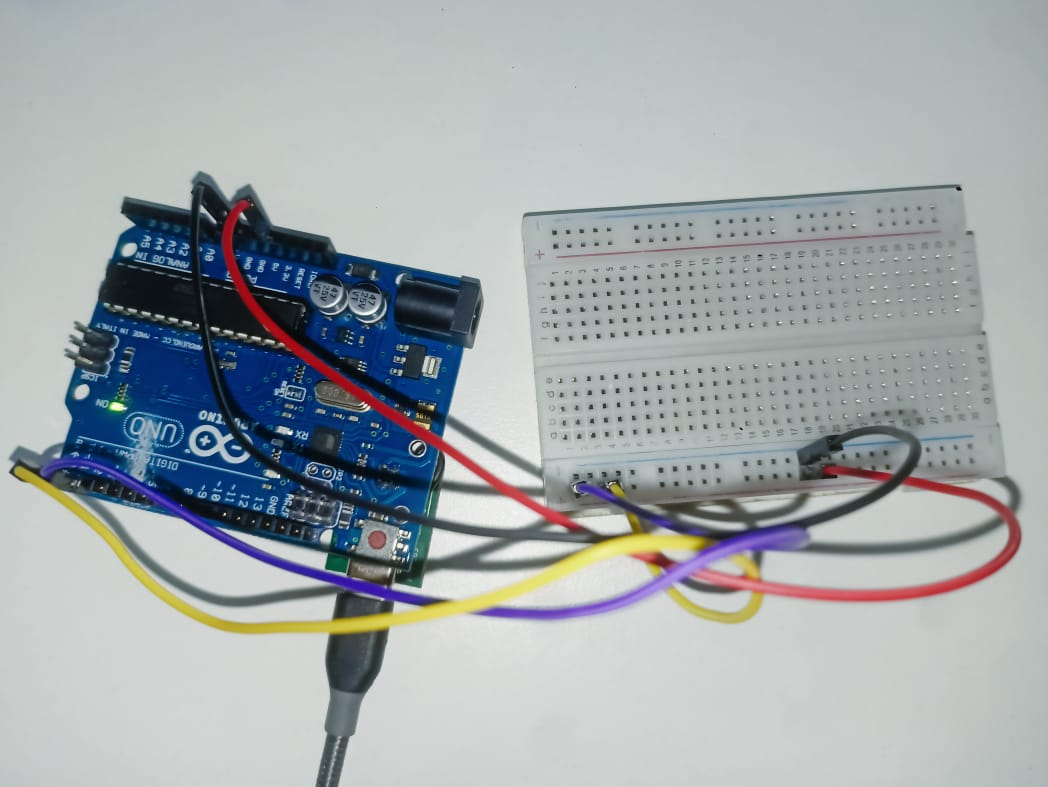
\includegraphics[width=0.3\columnwidth]{21-1.jpg}
		\caption{Connections}
		\label{fig:connections}
	\end{figure}
	\section{Software}
	Now write the code which is available in below path and upload to the Arduino. \\
	\framebox{https://github.com/Pavan2k01/Digital-Design/blob/main/Platformio/Platformio.cpp}
	\section{Conclusion}
	Hence, we have implemented the NOR gate for the given circuit in ide environment with the help of Arduino.
\end{document}
